\documentclass[12pt]{article}
\usepackage[a4paper, margin=1in]{geometry}
\usepackage[T1]{fontenc}
\usepackage{graphicx}
\usepackage{titlesec}
\usepackage{caption}
\usepackage{subcaption}
\usepackage[section]{placeins}
\usepackage{chngcntr}
\usepackage{sectsty}
\usepackage{algorithmicx}
\usepackage[ruled,vlined]{algorithm2e}
\usepackage[hidelinks]{hyperref}
\usepackage{listings}
\usepackage{xcolor}
\usepackage{amsmath}

\sectionfont{\centering}
\counterwithin{figure}{section}
\renewcommand{\abstractname}{\large Abstract}
\renewcommand{\baselinestretch}{1.5}

\lstset{
    basicstyle=\ttfamily,
    columns=fullflexible,
    breaklines=true,
    postbreak=\mbox{\textcolor{red}{$\hookrightarrow$}\space}
}

\newcommand{\sectionfontstyle}{\fontsize{16pt}{1em}\usefont{T1}{phv}{b}{n}}

\begin{document}
    \pagenumbering{gobble}
    \thispagestyle{empty}
    \begin{center}
        \textit{Project Report on}\\
        \vspace{2mm}
        \Large{\textsc{Sql2Neo: Interconversion of SQL, NoSQL and Neo4j formats}}\\
        \vspace{3mm}
        \textit{Submitted by}\\
        \large{\textbf{
            Aayush Jain (16IT101)\\
            Aditi Rao (16IT103)
        }}\\
        \vspace{4mm}
        Under the Guidance of\\
        \textbf{Shruti J R}\\
        Department of Information Technology, NITK Surathkal\\
        \vspace{4mm}
        \textit{Date of Submission: 11 June 2020}\\
        \vspace{4mm}
        in partial fulfillment for the award of the degree\\
        of\\
        \textbf{Bachelor of Technology}\\
        In\\
        \textbf{Information Technology}\\
        At
        \vspace{4mm}\\
        
\includegraphics[width=1.2in,height=1.2in]{img/nitk.jpg}\\
        \textbf{Department of Information Technology}\\
        \textbf{National Insitute of Technology Karnataka, Surathkal}\\
        June 2020
    \end{center}

    \newpage

    \begin{abstract}
        In order to leverage data relationships and gain insights into the ``big picture'' presented by the data, organizations need a database technology that stores relationship information as a first-class entity. This can be done through the use of Graph Databases such as Neo4j. However, many legacy databases are currently stored in SQL or (more recently) non-graphical NoSQL based systems which thus removes the possibility of enhanced insights brought about through the use of a graph. Thus, this work details the methodology and implementation of Sql2Neo, a command line tool to convert data between SQL/NoSQL systems to Neo4j. The resulting database does not only effectively store data relationships; but is also flexible when expanding a data model or conforming to changing business needs, and is uniquely suited to visualization for higher level decision making and inference mining. In addition, Sql2Neo also supports query translation to Neo4j’s Cypher Query Language (CQL) from standard formats such as SQL, increasing the ease of mobility from SQL/NoSQL systems to Neo4j without the rewriting of existing queries. 
    \end{abstract}

    \newpage

    \tableofcontents

    \newpage

    \pagenumbering{arabic}

    \section{\sectionfontstyle Introduction}
    A graph database is an online database management system with Create, Read, Update and Delete (CRUD) operations working on a graph data model. A graph data model is defined by a collection of nodes which represent entities and  relationships that connect the nodes. Graph databases are preferred when we want to focus exclusively on understanding the relationship between entities in our database, and want to be able to infer data connections without using things like foreign keys or out-of-band processing, such as MapReduce. 

    In order to leverage data relationships and gain insights into the ``big picture'' presented by the data, organizations need a database technology that stores relationship information as a first-class entity. The rigid schemas of legacy relational database management systems (RDBMS) make it difficult to add different connections or adapt to new business requirements. Not only do graph databases effectively store data relationships; they’re also flexible when expanding a data model or conforming to changing business needs, and are uniquely suited to visualization for higher level decision making and inference mining.

    Relational Databases or SQL databases are a  type of DBMS that defines database relationships in the form of tables, also known as relations and are the most popular DBMS type in the market. Unlike network DBMS, RDBMS does not support many to many relationships.Relational DBMS usually have pre-defined data types that they can support. SQL stands for Structured Query language, and is the standard language for dealing with Relational Databases.It can be used to insert, search, update and delete database records as well as lots of other operations including optimizing and maintenance of databases. Databases like MySQL Database, Oracle, Ms SQL server, Sybase, etc use SQL.

    NoSQL is an upcoming category of Database Management Systems. It’s main characteristic is it’s non-adherence to Relational Database Concepts. The popularity of NoSQL databases grew with internet giants such as Google, Facebook, Amazon etc who use them to deal with gigantic volumes of data. NoSQL systems are preferred in these cases as when you use a relational database for massive volumes of data , the system starts getting slow in terms of response time. The alternative to upgrading hardware to fix the problem would be to distribute our database load on multiple hosts as the load increases. This is known as "scaling out". NOSQL databases are non-relational databases that scale out better than relational databases and are designed with web applications in mind. They do not use SQL to query the data and do not follow strict schemas like relational models. Some examples of NoSQL databases include MongoDB, CouchDB and HBase.
    Neo4j is a graph database management system described as an ACID-compliant transactional database with native graph storage and processing. Neo4j is the most popular graph database used today. Neo4j is implemented in Java and accessible from software written in other languages using CQL through a transactional HTTP endpoint, or through the binary ``bolt'' protocol.

    \newpage

    \section{\sectionfontstyle Literature Survey}
    \subsection{Related Work}
    Singh et al.~\cite{base_paper} propose a methodology to convert a relational to a graph database by exploiting the schema and the constraints of the source, applied in this case to healthcare data. In this work MySQL as a relational database and Neo4j as a graph database was used for the implementation of the proposed system. They reported the notable efficiency of the system designed for querying. They also note that visualization has also significantly improved with the usage of graph databases.

    De Virgilio et al.~\cite{rdbms2graph} also propose a methodology to convert a relational database to a graph database by exploiting the schema and the constraints of the source. The approach also supports the translation of conjunctive SQL queries over the source into graph traversal operations over the target. The methodology describes an automatic conversion system from SQL databases to a graph database which allows the created database to perform better than RDB in certain instances of highly complicated schemas.

    Maity et al.~\cite{nosql2rdbms} view the standard problem of converting the RDBMS to NoSQL in reverse approach and conceptualize a problem where NoSQL is converted back to a RDBMS based system.  The approach is illustrated using a case study on MongoDB and Neo4j. They note significant successes in conversion using their algorithm and note the potential for its use in not only  NoSQL systems to RDBMS, but also for interconversion between two NoSQL systems.

    Vicknair et al.~\cite{db_comparison} report on a comparison of Neo4j with MySQL, for use as the underlying technology in the development of a software system to record and query data provenance information. They noted an almost tenfold increase in speed while using Neo4j for traversal based queries. They conclude that in general, the graph database did better at the structural type queries and full-text character searches than the relational database, and that with more development of Neo4j to include integer based indexing measures as well, it could outperform RDBMS systems in a query on numeric data.

    Batra and Tyagi~\cite{rgdb_compare} also report on the comparative performance of Neo4j and MySQL, noting that the retrieval times of graph databases is less than relational databases as  graph databases look only at records that are directly connected to other records. They conclude noting the flexibility of graph databases when new relationships are added as schema restructuring is not required.

    \subsection{Outcome of Literature Survey}
    From the survey, it is clear that the use of graph dbs for applications involving great focus on entity relationships or visualization would be highly beneficial. It is also evident that it may be useful to transform data from traditional RDBMS to NoSQL systems such as graph databases simply for the flexibility it offers in terms of addition of relationships/query speeds for traversal queries. Our proposed methodology aims to allow for quick and easy transformation of existing databases to graph format to take advantage of these benefits. 

    \subsection{Problem Statement}
    Graph databases systems such as Neo4j offer various advantages over traditional RDBMS in terms of traversal queries, visualization as well as flexibility in defining new relations without schema restructuring. However, a vast majority of applications that could benefit from this store data in traditional SQL setups (while some do in newer, NoSQL systems). Thus, there is a need to develop a tool to allow for efficient transformation between these systems to graph databases to enhance decision making and insights into the data.

    \subsection{Objectives}
    In order to meet the demands of this problem, our proposed system must meet the following objectives. The system architecture must be designed to allow for \textit{extensibility}, in terms of addition of new SQL/NoSQL systems to convert from. To allow for this it is necessary to develop a \textit{standard intermediate format} from which conversion to Neo4j can take place. The system must be able to accurately and appropriately \textit{represent relationships} expressed by the use of concepts such as foreign keys in RDBMS, as well as the many to many relationships described in NoSQL systems. The transformation must be done quickly, \textit{without loss of information} and into a form suitable for direct visualization. There must also be an efficient method for \textit{query translation from SQL/NoSQL based query languages to CQL}, as well as creation of required indices on identified fields to allow for faster query processing and result retrieval.

    \newpage

    \section{\sectionfontstyle Requirement Analysis}
    Sql2Neo is intended to be a command line tool that enables interconversion between SQL, NoSQL and Neo4j formats.

    \subsection{Functional Requirements}
    \begin{enumerate}
        \item [F1.] SQL databases must be fully converted to a Neo4j database. This includes indexes, constraints, records and relationships.
        \item [F2.] NoSQL databases must be fully converted to a Neo4j database. This includes constraints (inferred) and records.
        \item [F3.] SQL queries must be translated to a Neo4j query to provide interoperability between databases.
    \end{enumerate}

    \subsection{Non-Functional Requirements}
    \begin{enumerate}
        \item [NF1.] Convert NoSQL database to intermediate SQL format to provide compatibility.
        \item [NF2.] Manage data loading from databases in order to prevent memory overuse and overflow errors.
        \item [NF3.] Provide Sql2Neo as an isolated tool (with packaged dependencies) to improve usability.
    \end{enumerate}

    Most software and hardware requirements intersect with the implementation tools, as discussed in section~\ref{sec:impl}.

    \newpage

    \section{\sectionfontstyle System Design/Architecture}
    \label{sec:sys_arch}
    \begin{figure}[htb!]
        \centering
        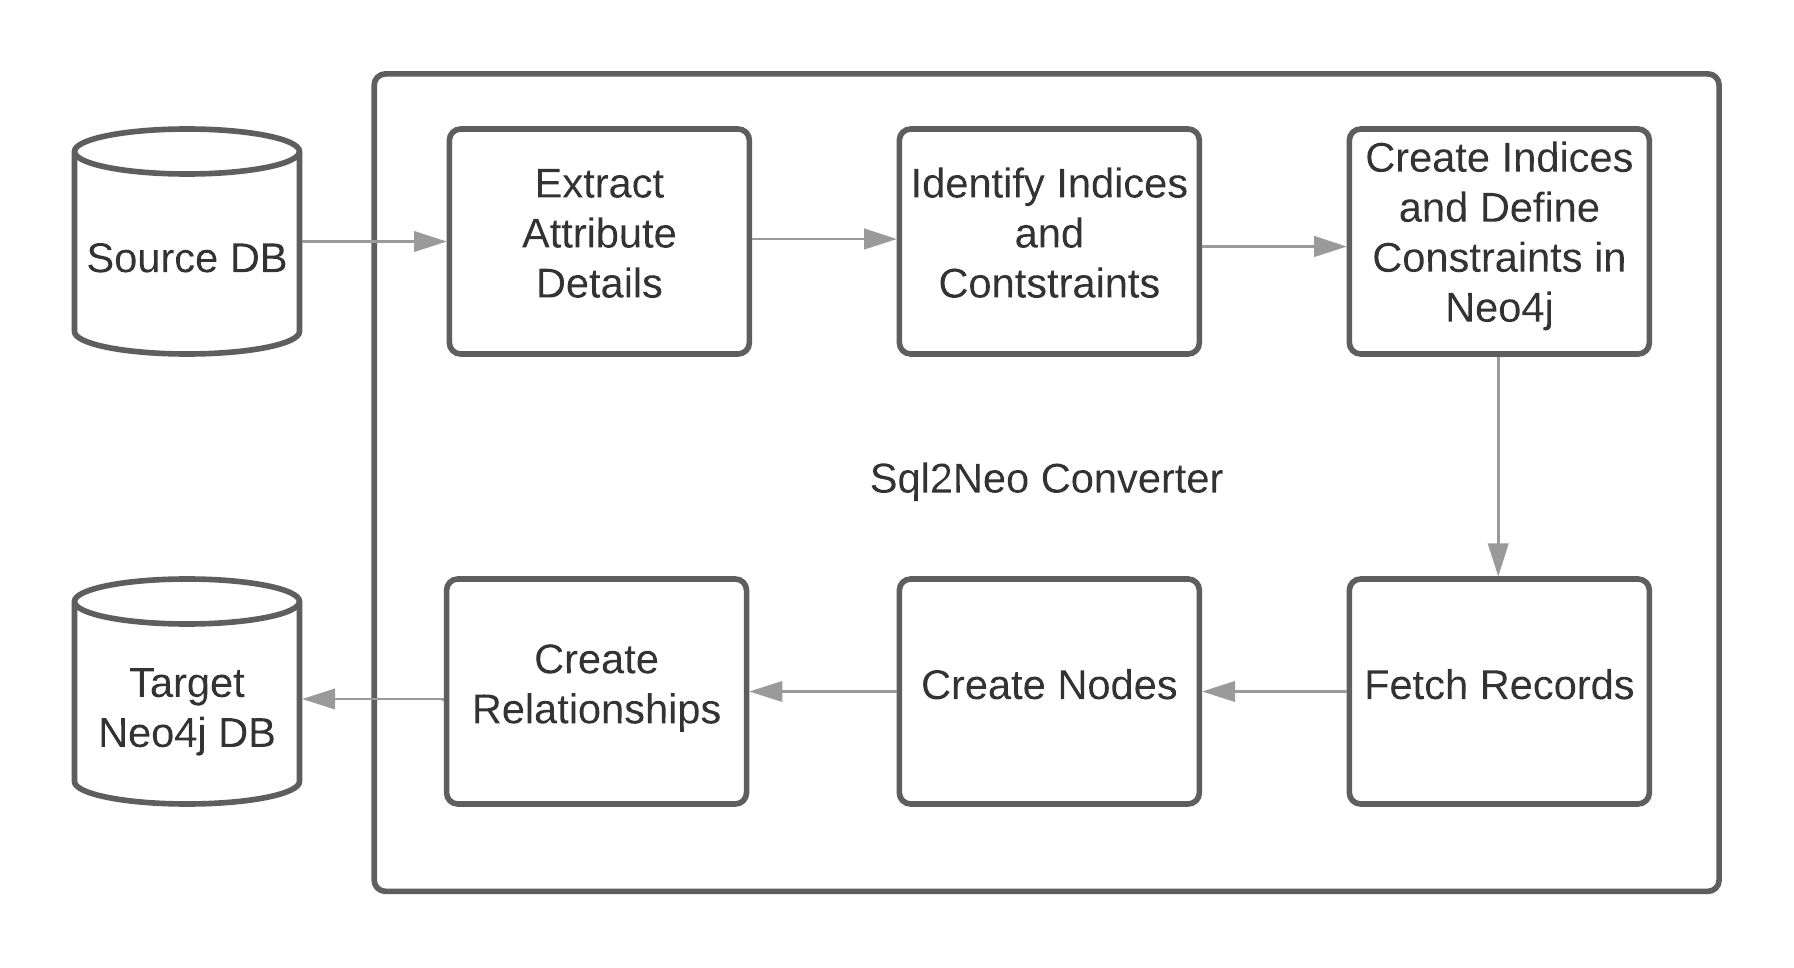
\includegraphics[width=155mm]{img/sql2neo_converter.png}
        \caption{SQL2Neo Data Converter}
        \label{fig:sql2neo_converter}
    \end{figure}

    Figure~\ref{fig:sql2neo_converter} presents an overview of the proposed system architecture. The aim is to take our source database and start by extracting attribute details. This includes information on attribute name, datatype (in case conversion is required as Neo4j does not support some data types), uniqueness, if it is a primary/foreign key or if an index needs to be built on it. Through this we can then further identify indices and constraints in the data, and subsequently define them as required. At the end of this step, all data description  information has been translated to a format which can be further used while translating records into Neo4j.

    Then we begin the population of the Neo4j database. We fetch the records from the source database and, using the data descriptions we have extracted in the previous steps, store it in an intermediate, universal format. This is the last step before node and relationship creation in Neo4j begins.
    
    As Neo4j creates relationships between existing nodes, the nodes are defined first from the identified entities in the data description. Then, relationships or links between the nodes are created and committed to the database.
    
    The system architecture has been designed to encourage extensibility to include compatibility with multiple SQL and NoSQL implementations. All the primary steps before node creation begins deal with bringing the data to an established universal format after which conversion to Neo4j entities and relationships is a single pipeline process for all. Thus, it requires that only translation steps to this intermediate format must be determined to include another implementation in the converter.
    
    \begin{figure}[htb!]
        \centering
        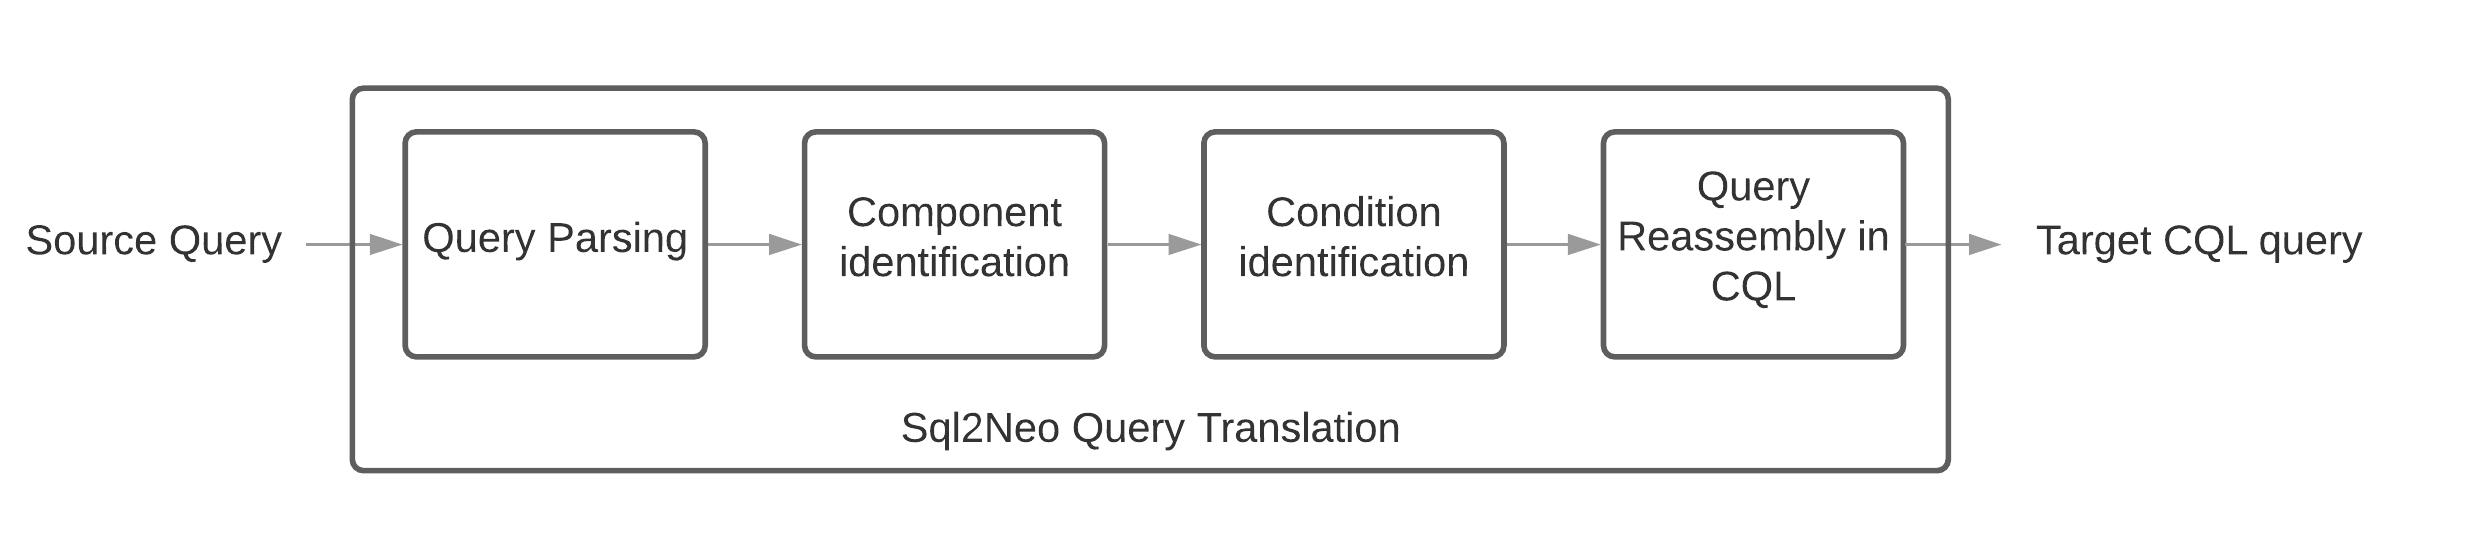
\includegraphics[width=155mm]{img/sql2neo_query.png}
        \caption{SQL2Neo Query Translator}
        \label{fig:sql2neo_query}
    \end{figure}

    In addition, we also undertake query translation from source (SQL/NoSQL) to CQL or Cypher Query Language. The steps begin with parsing the query to isolate terms of interest (figure~\ref{fig:sql2neo_query}). This is followed by identifying components (such as entities and attributes) from the parsed data. We then identify any conditional clauses to be placed (such as found in an SQL “WHERE” query phrase) and represent them appropriately. Finally, the Query is reassembled from its components and placed into a template structure for an equivalent CQL query.

    \newpage

    \section{\sectionfontstyle Methodology}
    \subsection{Converting SQL-databases to Neo4j format}
    The first step to convert an SQL database is to extract attribute details of each table. This data is available in the \verb|information_schema| of the database. The data for each attribute answers the following questions:
    \begin{itemize}
        \item should this attribute be \textit{indexed}?
        \item does this attribute have a \textit{uniqueness constraint}?
        \item is this attribute a \textit{foreign key reference} to another table's attribute?
    \end{itemize}

    \begin{algorithm}[htb!]
        \SetAlgoLined
        \label{algo:sql_attr_extract}
        \caption{Extract attribute details of SQL database}
        \KwIn{\textbf{R}, a relational database}
        \KwOut{\textbf{AS}, an attribute set containing details of each attribute}
        AS \gets\ \phi\tcc*{empty map}
        \ForEach{table in \textbf{information\_schema(R)}}{
            AS[table] \gets\ \phi\tcc*{empty map}
            \ForEach{attr in \textbf{table}}{
                AS[table][attr] \gets\ \{index, unique, fk\}\;
            }
        }
        return AS\;
    \end{algorithm}

    The index and uniqueness constraint data enable the Neo4j setup to be as closely modelled to the relational one. Furthermore, indexing on attributes is maintained across systems and rigid constraints are also satisfied while inserting in the Neo4j database.

    Since Neo4j stores data as JSON documents, it does not define a rigid and formal schema. Owing to this property, indices and constraints can be created before the data is actually inserted. In Neo4j, index creation is not idempotent, meaning that creating the index twice reults in an error. Additionally, constraints implicitly create an index on the specified attribute (much like relational databases), thus constraints are applied only on those attributes that are not indexed.

    \begin{algorithm}[htb!]
        \SetAlgoLined
        \label{algo:sql_create_index}
        \caption{Create indices and constraints in Neo4j}
        \KwIn{\textbf{AS}, an attribute set containing details of each attribute}
        \KwResult{\textbf{G}, a graph database with applied indices and constraints}
        \ForEach{table in \textbf{AS}}{
            \ForEach{attr in \textbf{table}}{
                \uIf{attr must be indexed}{
                    CreateIndex(G, table, attr)\;
                }
                \uElseIf{attr has constraint but not indexed}{
                    \tcc*[h]{if attr is indexed, then it meets uniqueness constraint}

                    CreateUniquenessConstraint(G, table, attr)\;
                }
            }
        }
    \end{algorithm}

    In terms of Cypher Query Language (CQL), \verb|CreateIndex(G, table, attr)| is equivalent to 
    \begin{lstlisting}
        CREATE INDEX index_name ON:table(attr);
    \end{lstlisting}
    \verb|CreateUniquenessConstraint(G, table, attr)| is equivalent to 
    \begin{lstlisting}
        CREATE CONSTRAINT constraint_name ON (t:table) ASSERT t.attr IS UNIQUE;
    \end{lstlisting}

    Conversion of a table's records to Neo4j nodes is a fairly straightforward task. A naive approach is followed where each tables records are converted to a node. This implies that certain tables that behave purely as relationships are also converted to nodes instead of being retained into Neo4j.

    \begin{algorithm}[htb!]
        \SetAlgoLined
        \label{algo:sql2graph}
        \caption{Populate the graph database with records}
        \KwIn{\textbf{R}, a relational database}
        \KwResult{\textbf{G}, a populated graph database}
        \ForEach{table in \textbf{R}}{
            \ForEach{record in \textbf{table}}{
                CreateNewNode(G, table, record)\;
            }
        }
    \end{algorithm}

    \verb|CreateNewNode(G, table, record)| is equivalent to 
    \begin{lstlisting}
        CREATE (t:table $record);
    \end{lstlisting}
    provided that \verb|record| is a map of key-value pairs (record assumed as a parameter).

    Finally, relationship conversion is performed. This step takes the foreign key relations from each table and maps them to a relation in Neo4j. This also means that the semantics of the relation are lost since the edge (in Neo4j) does not provide actual data. Rather it must be inferred from the database.

    \begin{algorithm}[htb!]
        \SetAlgoLined
        \label{algo:sql2rel}
        \caption{Create relationships between nodes in the graph data}
        \KwIn{\textbf{AS}, an attribute set containing details of each attribute}
        \KwResult{\textbf{G}, a graph database with relationships}
        \ForEach{table in \textbf{AS}}{
            \ForEach{attr in \textbf{table}}{
                \If{attr is foreign key}{
                    fk\_table, fk\_attr \gets\ GetFKReference(attr)\;
                    CreateRelationship(G, table, attr, fk\_table, fk\_attr)\;
                }
            }
        }
    \end{algorithm}

    \verb|CreateRelationship(G, table, attr, fk_table, fk_attr)| is equivalent to 
    \begin{lstlisting}
        MATCH (a:table), (b:fk_table) WHERE a.attr = b.fk_attr CREATE (a) -[r:relationship_name]-> (b);
    \end{lstlisting}

    \clearpage

    \section{\sectionfontstyle Implementation}
    \label{sec:impl}
    The proposed approach was implemented on a system running Ubuntu 20.04 LTS. The following additional software is used:
    \begin{itemize}
        \item Python 3.8.2
        \begin{itemize}
            \item mysql-connector-python 8.0.20
            \item py2neo 4.3.0
            \item pymongo 3.10.1
            \item python-dotenv 0.13.0
            \item pandas 1.0.4
        \end{itemize}
        \item MySQL v8.0.20 for testing SQL databases
        \item MongoDB v3.6.8 for testing NoSQL databases
        \item Neo4j 4.0.5
    \end{itemize}

    \newpage

    \section{\sectionfontstyle Results and Analysis}
    Results

    \newpage

    \section{\sectionfontstyle Conclusion and Future Works}
    In conclusion, it is found that it is not only feasible to undertake such transformation tasks between SQL/NoSQL databases, but that it is also quite beneficial when considering improved data visualization and presentation. The implementation of Sql2Neo discussed is additionally easily extensible to include various other source databases as a result of its system architecture and the use of an intermediate SQL -like data storage strategy. 

    Future works include, as mentioned, the extension of this project to bring more source databases within the transformation fold, as well as to improve the quality of relationships derived from the data through more inference driven approaches (rather than the naive approach undertaken here). 

    \newpage

    \bibliographystyle{ieeetr}
    \bibliography{references}
\end{document}